% Copyright (c) 2014,2016 Casper Ti. Vecto
\chapter{系統實現}

% \section{區塊鏈的實名交易監督系統實現}

為了驗證和證明所提議的BRTMS用於比特幣支付收款監督的可行性和有效性,我們將其運行在用於商家商品管理和維護的Java應用程序的SMIMSS子系統,用於商家職員的運行在Android App上的SMCTSS以及運行在App上的用於客戶的CMPTSS。
如圖\ref{fig5}所示,SMIMSS Java應用程序可以幫助商家登錄到系統或創建一個新帳戶。 授權商戶成功登錄系統後,商家可以插入或更新產品列表,如圖\ref{fig6}所示。實施的SMIMSS Java應用程序執行前面部分中所述的功能。

\begin{figure}[htbp]
	\centering
	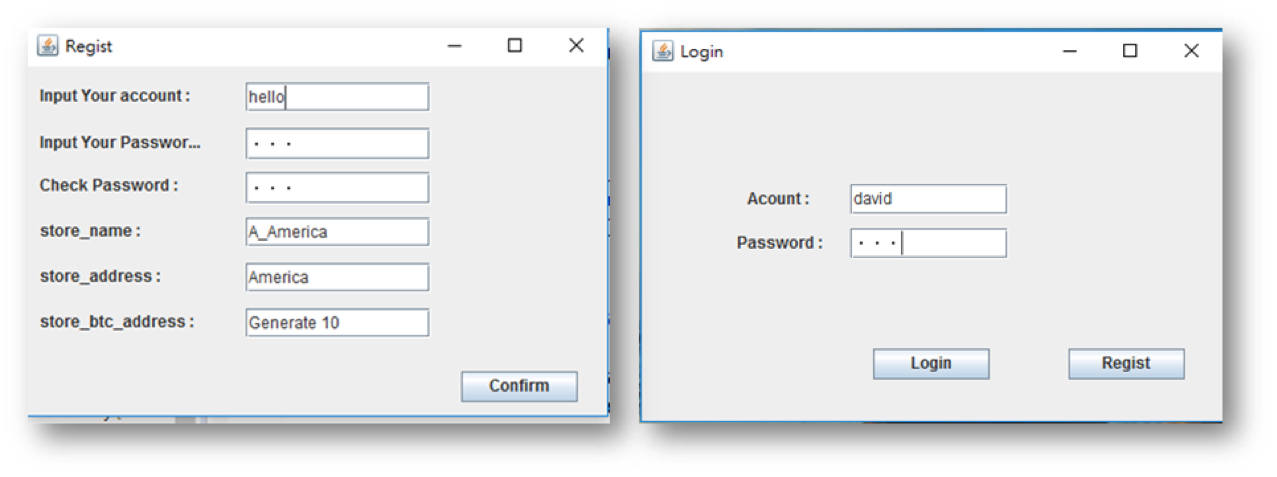
\includegraphics[width = 0.9\textwidth]{fig5.png}
	\caption{SMIMSS的Java應用程序的註冊和登錄界面}\label{fig5}
\end{figure}

\begin{figure}[htbp]
	\centering
	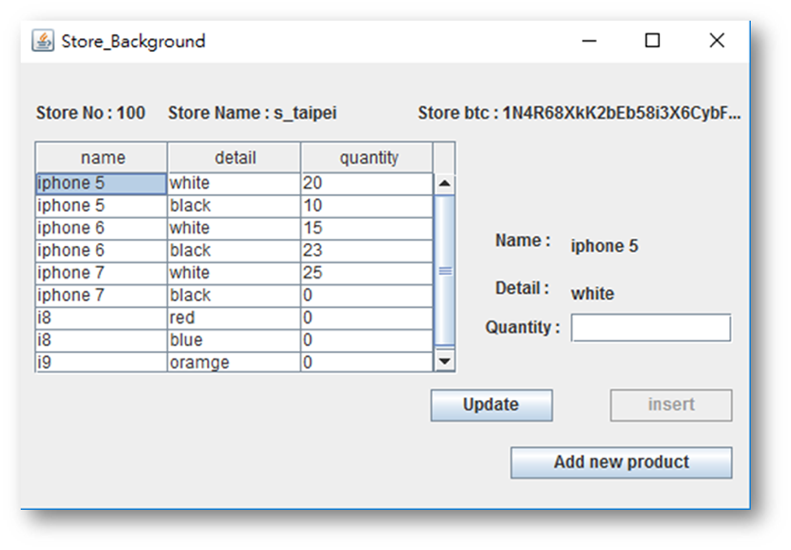
\includegraphics[width = 0.6\textwidth]{fig6.png}
	\caption{在SMIMSS中插入或更新授權商家的產品目錄}\label{fig6}
\end{figure}

商戶的產品信息可以通過RFID標籤掃描,存儲到雲端數據庫中,商戶店員可以使用我們實現的SMCTSS Android客戶端,啟用NFC監聽器,從購物車中的客戶購買產品中讀取RFID標籤信息。 在如圖\ref{fig7}所示的第一項活動中,商家職員必須登錄才能獲得授權訪問SMCTSS功能。 然後,在第二項活動中,SMCTSS應用程序可以通過使用SMIMSS中應用的雲數據庫檢查產品RFID標籤信息並將其展示給客戶,從而將掃描的產品列入購物車。 在圖\ref{fig7}的第三項活動中,顧客可以要求店員取消購買物品以確認最終購買。 最後,SMCTSS應用程序將自動使用比特幣測試網絡(Bitcoin Testnet)\supercite{bitcointestnet}幫助店員確認發布此加密貨幣交易的收款人地址,如圖\ref{fig7}所示。    

\begin{figure}[htbp]
	\centering
	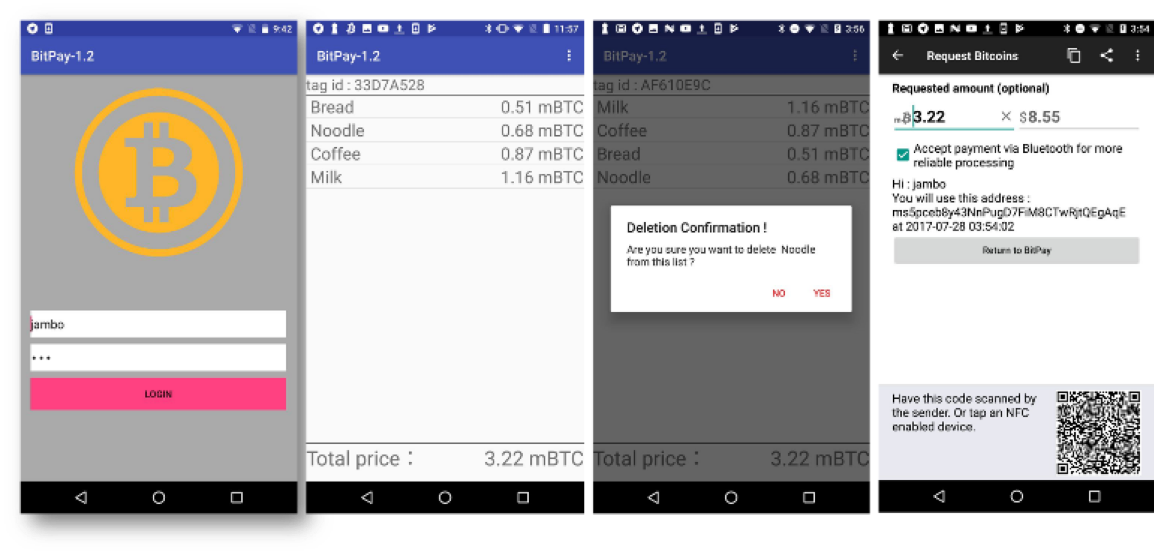
\includegraphics[width = 1\textwidth]{fig7.png}
	\caption{登錄、等待結帳的商品、刪除商品及支付確認}\label{fig7}
\end{figure}

同時,客戶將使用與SMCTSS App相對應的CMPTSS Android App通過比特幣加密貨幣完成採購產品交易。 如圖\ref{fig8}所示,第一個活動表示顧客確認購買產品創建交易數據庫的交易清單,第二個活動顯示包括金額和付款人比特幣地址在內的付款確認,第三個活動顯示交易歷史記錄 的交易作為買方甚至是賣方,最後在第四項活動中顯示了該筆交易詳細採購產品的發票。    

\begin{figure}[htbp]
	\centering
	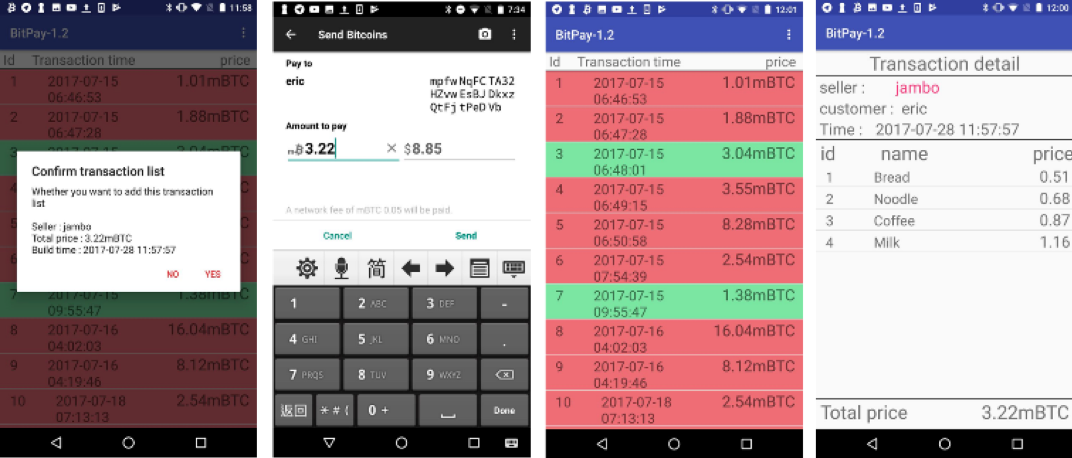
\includegraphics[width = 1\textwidth]{fig8.png}
	\caption{在CMPTSS App中,交易確認,付款確認、交易歷史記錄和發票}\label{fig8}
\end{figure}